%%%%%%%%%%%%%%%%%%%%%%%%%%%%%%%%%%%%%%%%%
% Beamer Presentation
% LaTeX Template
% Version 1.0 (10/11/12)
%
% This template has been downloaded from:
% http://www.LaTeXTemplates.com
%
% License:
% CC BY-NC-SA 3.0 (http://creativecommons.org/licenses/by-nc-sa/3.0/)
%
%%%%%%%%%%%%%%%%%%%%%%%%%%%%%%%%%%%%%%%%%

%----------------------------------------------------------------------------------------
%	PACKAGES AND THEMES
%----------------------------------------------------------------------------------------

\documentclass{beamer}

\mode<presentation> {

% The Beamer class comes with a number of default slide themes
% which change the colors and layouts of slides. Below this is a list
% of all the themes, uncomment each in turn to see what they look like.

%\usetheme{default}
%\usetheme{AnnArbor}
%\usetheme{Antibes}
%\usetheme{Bergen}
%\usetheme{Berkeley}
%\usetheme{Berlin}
%\usetheme{Boadilla}
%\usetheme{CambridgeUS}
%\usetheme{Copenhagen}
%\usetheme{Darmstadt}
%\usetheme{Dresden}
%\usetheme{Frankfurt}
%\usetheme{Goettingen}
%\usetheme{Hannover}
%\usetheme{Ilmenau}
%\usetheme{JuanLesPins}
%\usetheme{Luebeck}
%\usetheme{Madrid}
%\usetheme{Malmoe}
%\usetheme{Marburg}
%\usetheme{Montpellier}
%\usetheme{PaloAlto}
%\usetheme{Pittsburgh}
%\usetheme{Rochester}
%\usetheme{Singapore}
%\usetheme{Szeged}
%\usetheme{Warsaw}

% As well as themes, the Beamer class has a number of color themes
% for any slide theme. Uncomment each of these in turn to see how it
% changes the colors of your current slide theme.

%\usecolortheme{albatross}
%\usecolortheme{beaver}
%\usecolortheme{beetle}
%\usecolortheme{crane}
%\usecolortheme{dolphin}
%\usecolortheme{dove}
%\usecolortheme{fly}
%\usecolortheme{lily}
%\usecolortheme{orchid}
%\usecolortheme{rose}
%\usecolortheme{seagull}
\usecolortheme{seahorse}
%\usecolortheme{whale}
%\usecolortheme{wolverine}

%\setbeamertemplate{footline} % To remove the footer line in all slides uncomment this line
%\setbeamertemplate{footline}[page number] % To replace the footer line in all slides with a simple slide count uncomment this line

%\setbeamertemplate{navigation symbols}{} % To remove the navigation symbols from the bottom of all slides uncomment this line
}
\usepackage{media9}
\usepackage{graphicx} % Allows including images
\usepackage{booktabs} % Allows the use of \toprule, \midrule and \bottomrule in tables
\usepackage{cite}
 \usepackage{multimedia}
\setbeamertemplate{navigation symbols}{}
\setbeamertemplate{bibliography item}{\insertbiblabel}
\setbeamertemplate{frametitle continuation}[from second]
%----------------------------------------------------------------------------------------
%	TITLE PAGE
%----------------------------------------------------------------------------------------

\title[] {Continues Integration Pipeline Implementation
for Tech11Software}
\author[]{Aswin Sugu\\Jefin Jacob\\Nitin Suresh\\Vishnu Bose\\Guided By\\Mrs. Greeshma N Gopal \\Asst.Professor in CSE}
\institute[CE CHERTHALA]{COLLEGE OF ENGINEERING CHERTHALA}
\date{\today}
%\date{8/8/16} % Date, can be changed to a custom date

\begin{document}

\begin{frame}
\titlepage % Print the title page as the first slide
\end{frame}

\begin{frame}
\frametitle{Overview} % Table of contents slide, comment this block out to remove it
\tableofcontents % Throughout your presentation, if you choose to use \section{} and \subsection{} commands, these will automatically be printed on this slide as an overview of your presentation
\end{frame}

%----------------------------------------------------------------------------------------
%	PRESENTATION SLIDES
%----------------------------------------------------------------------------------------
% Sections can be created in order to organize your presentation into discrete blocks, all sections and subsections are automatically printed in the table of contents as an overview of the talk
%------------------------------------------------

%\subsection{} % A subsection can be created just before a set of slides with a common theme to further break down your presentation into chunks
%\subsection{Android System}


%\begin{frame}{Title}
%
% \includemedia[
%  width=\paperwidth,
%  height=0.7\linewidth,
%   activate=onclick,
%   deactivate=onclick,
% addresource=ero.mp4,
% flashvars={source=ero.mp4
% &loop=false
% &scaleMode=letterbox
%    }
% ]{\textsc{0.02in}{erotion}}{VPlayer.swf}
 

 
% \begin{center}
%\href{run:/usr/local/bin/mplayer -fs forced_pendulum.mp4}{
%\includegraphics[scale=0.25]
%{forced_pendulum.eps}}
%\end{center}
% \end{frame}


\section{AUTHOR}
\begin{frame}{AUTHOR}
\begin{itemize}
\item Proposed by Sourav Bhowmick, Sushant Kumar and Anurag Kumar
School of Engineering
Tezpur University
Tezpur, Assam-785024, India.

\end{itemize}
\end{frame}
%\section{Introduction}
\section{INTRODUCTION}
\begin{frame}{INTRODUCTION}
%\begin{itemize}
%\item 
\begin{block}{}
Hand gesture and hand posture differ in their
respective interpretation.
\end{block}

\vspace{.5 cm}
% \item
\begin{block}{}


 HCI(Human Computer Interaction) using Gesture and Sign language recognition (SLR), aimed at creating a virtual reality, 3D gaming environment, helping the deaf-and-mute people etc.,
extensively exploit the use of hand gestures.
\end{block}
%\begin{figure}
%\begin{center}
%\includegraphics[scale=0.5]{scene1.jpg}
%\caption{Scene Character }
%\end{center}
%\end{figure}


%\end{itemize}
\end{frame}
\begin{frame}{INTRODUCTION contd..}
%\begin{itemize}
\begin{block}{Gesture Recognition for Computer Games } 



\begin{figure}
\begin{center}
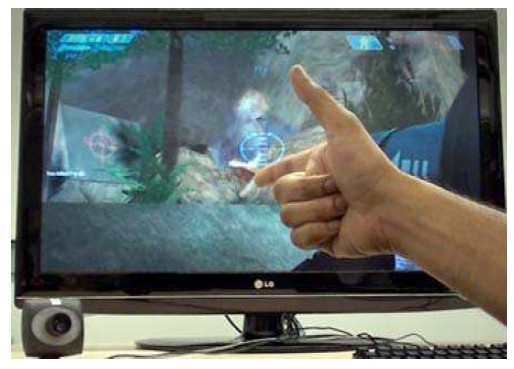
\includegraphics[scale=0.3]{images/game.jpg}
\caption{Controlling Games with Gestures }
\end{center}
\end{figure}

\end{block}
%\end{itemize}
\end{frame}
\begin{frame}{INTRODUCTION contd..}
%\begin{itemize}
\begin{block}{}


The Nintendo Wii is a big success because its motion-sensitive paddle lets users innovatively
control objects on the screen with hand gestures.
\end{block}
  \vspace{0.5cm}
 \begin{block}{}
Companies, such as GestureTek (www.gesturetek.com) and Oblong Indus-
tries (www.oblong.net), are currently developing the necessary hardware and software to track
hands and recognize hand gestures.
\end{block}
 \vspace{0.5cm}

%\end{itemize}
\end{frame}


\begin{frame}{INTRODUCTION contd..}
\begin{itemize}
\item Two types of Hand detection mechanism.
\begin{itemize}
\item Glove based
\begin{figure}
\begin{center}
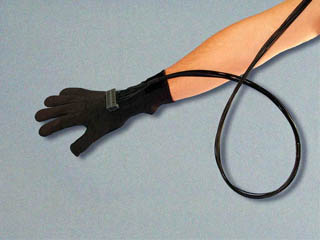
\includegraphics[scale=0.5]{images/glove.jpg}
%\caption{Example of scene character }
\end{center}
\end{figure}
\item Vision based
\begin{itemize}
\item Color based
\vspace{.5 cm}
\item Hand based
\end{itemize}
\end{itemize}


\end{itemize}
\end{frame}

\begin{frame}{INTRODUCTION contd..}
\begin{itemize}
\item Two types of Hand detection mechanism.
\begin{itemize}
\item Glove based
\begin{figure}
\begin{center}
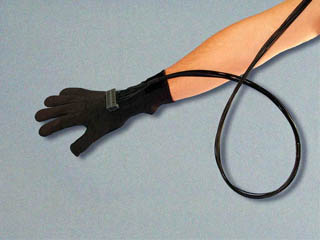
\includegraphics[scale=0.5]{images/glove.jpg}
%\caption{Example of scene character }
\end{center}
\end{figure}
\item \alert{Vision based}
\begin{itemize}
\item Color based
\vspace{.5 cm}
\item Hand based
\end{itemize}
\end{itemize}


\end{itemize}
\end{frame}

\begin{frame}{INTRODUCTION contd..}
\begin{itemize}
\item Color based
\begin{figure}
\begin{center}
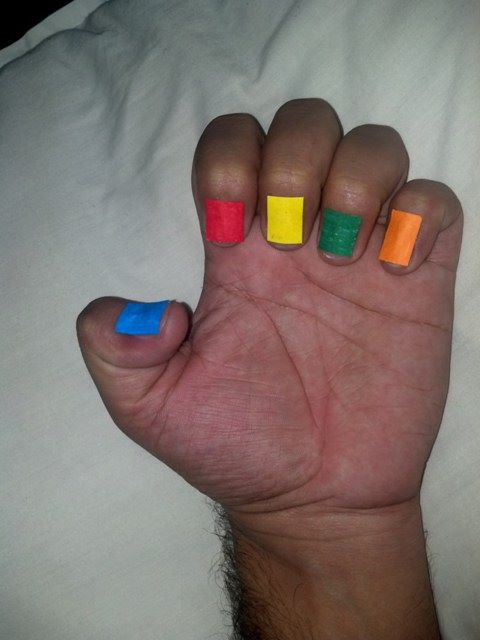
\includegraphics[scale=0.12]{images/colourhand.jpg}
%\caption{Example of scene character }
\end{center}
\end{figure}
\vspace{.5 cm}
\item Hand based
\begin{figure}
\begin{center}
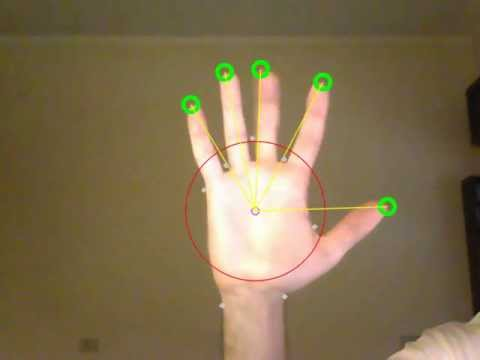
\includegraphics[scale=0.15]{images/plain.jpg}
%\caption{Example of scene character }
\end{center}
\end{figure}
 


\end{itemize}
\end{frame}


\begin{frame}{INTRODUCTION contd..}
\begin{itemize}
\item Color based
\begin{figure}
\begin{center}
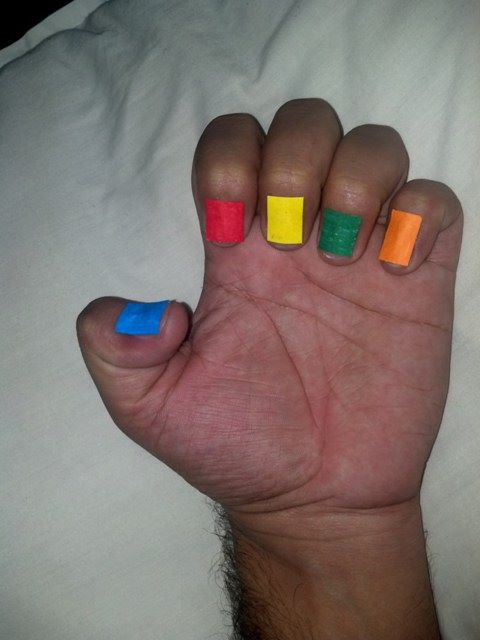
\includegraphics[scale=0.12]{images/colourhand.jpg}
%\caption{Example of scene character }
\end{center}
\end{figure}
\vspace{.5 cm}
\item \alert{Hand based}
\begin{figure}
\begin{center}
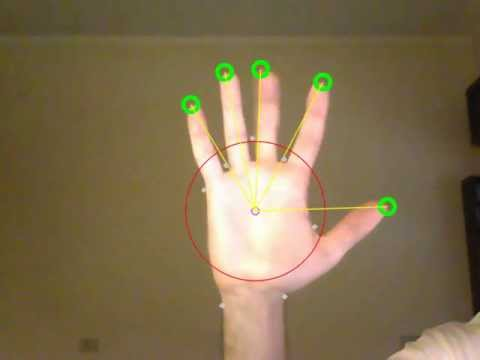
\includegraphics[scale=0.15]{images/plain.jpg}
%\caption{Example of scene character }
\end{center}
\end{figure}
 


\end{itemize}
\end{frame}

\begin{frame}{INTRODUCTION contd..}
\begin{itemize}
\item Hand Gestures for the English Alphabet
\begin{figure}
\begin{center}
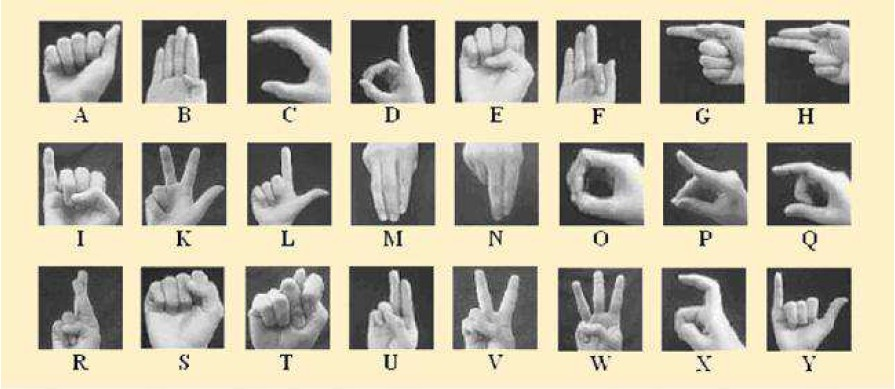
\includegraphics[scale=0.3]{images/alphabets.jpg}
%\caption{Example of scene character }
\end{center}
\end{figure}
\vspace{.5 cm}

%\item Recognizing
%isolated and continuous English alphabet gestures with artificial
%neural network with an objective to handling effectively
%the problems of similar gesture recognition and movements.
 


\end{itemize}
\end{frame}



\section{PROPOSED SYSTEM}
\begin{frame}{PROPOSED SYSTEM}
\vspace{0.5cm}
 \begin{itemize}
\item Any hand gesture recognition system requires some basic
stages. These stages are
\vspace{.5 cm}
 \begin{itemize}
\item Gesture module and image acquisition
\item Hand segmentation
\item Tracking
\item Feature extraction
\item Classification

\end{itemize}
\end{itemize}

%\movie{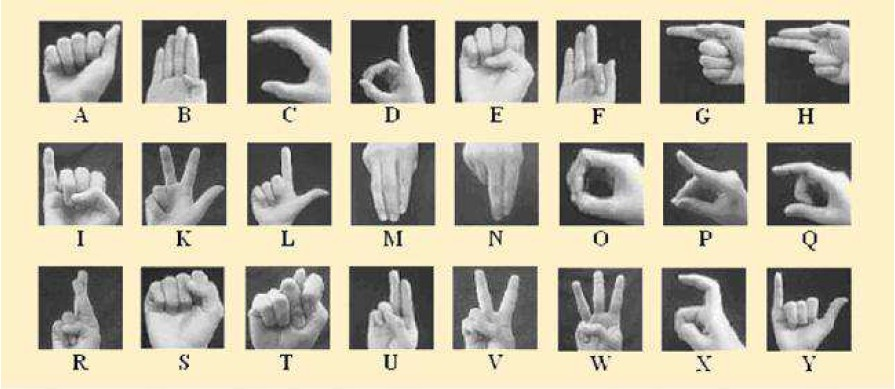
\includegraphics[width=0.2\textwidth]{images/alphabets.jpg}}{ero.mp3}
%
%\movie[width=9.1cm,height=6.5cm,showcontrols=true,loop,poster]{}{vbb.avi}
\end{frame}     

\begin{frame}{PROPOSED SYSTEM}
\vspace{0.5cm}
 \begin{itemize}
\item Any hand gesture recognition system requires some basic
stages. These stages are
\vspace{.5 cm}
 \begin{itemize}
\item \alert{Gesture module and image acquisition}
\item Hand segmentation
\item Tracking
\item Feature extraction
\item Classification

\end{itemize}
\end{itemize}
\end{frame}  

\begin{frame}{Gesture module and Image acquisition}
 \begin{itemize}
\item The video frames of the user is captured with the low-cost web-cam.
\begin{figure}
\begin{center}
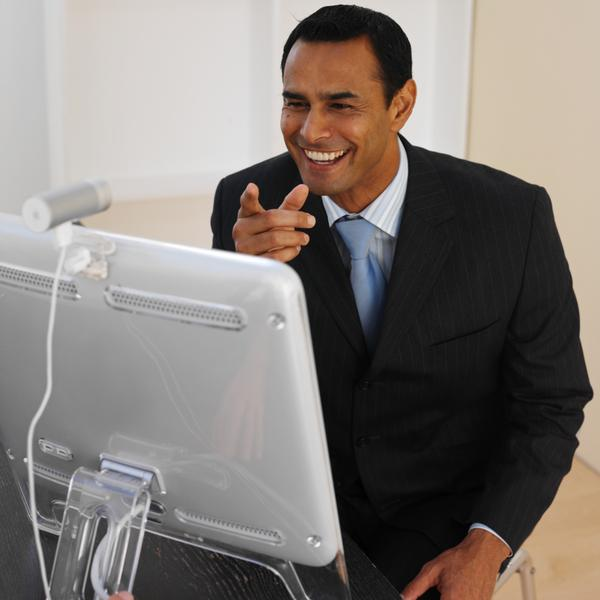
\includegraphics[scale=0.2]{images/webcam.jpg}
%\caption{Example of scene character }
\end{center}
\end{figure}
\vspace{.5 cm}


\end{itemize}
\end{frame}

\begin{frame}{Gesture module and Image acquisition}
 \begin{itemize}
\item The video frames is captured by a necessary Computer vision library[2].


\vspace{.5 cm}

\item Here the system processes have been captured at a resolution of 720x480 at 40 frames.
per second (fps).
\end{itemize}
\end{frame}

\begin{frame}{PROPOSED SYSTEM}
\vspace{0.5cm}
 \begin{itemize}
\item Any hand gesture recognition system requires some basic
stages. These stages are
\vspace{.5 cm}
 \begin{itemize}
\item Gesture module and image acquisition
\item \alert{Hand segmentation}
\item Tracking
\item Feature extraction
\item Classification

\end{itemize}
\end{itemize}
\end{frame} 

\begin{frame}{Hand Segmentation}
 \begin{itemize}
\item Proper hand segmentation from other body parts and
background is very crucial for the overall efficacy and the
effectiveness of any vision based hand gesture recognition.
\vspace{0.5 cm}
\item Skin colour based segmentation is used.
  

   

\end{itemize}
\end{frame}



\begin{frame}{Hand Segmentation}
 \begin{itemize}
 \item Here the Hand must separated from the rest of the body parts and from the surrounding.
 \item For proper segmentation, the user must worn a full sleeve black dress to separate hand from other body parts.
  
 \begin{figure}
  \begin{center}
  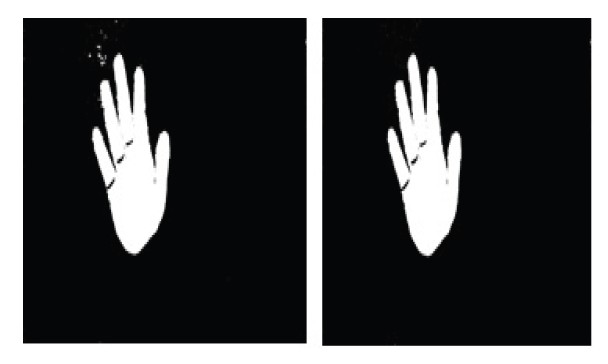
\includegraphics[scale=0.2]{images/segment.jpg}
  %\caption{sec }
  \end{center}
  \end{figure} 
  
\end{itemize}
\end{frame}

\begin{frame}{PROPOSED SYSTEM}
\vspace{0.5cm}
 \begin{itemize}
\item Any hand gesture recognition system requires some basic
stages. These stages are
\vspace{.5 cm}
 \begin{itemize}
\item Gesture module and image acquisition
\item Hand segmentation
\item \alert{Tracking}
\item Feature extraction
\item Classification

\end{itemize}
\end{itemize}
\end{frame} 

\begin{frame}{Hand Tracking}
\begin{itemize}
\item technique which
constantly monitors the consecutive positions/locations of the
region of interest (ROI) (hand in this case). 
\linebreak
\item To find the
gesture trajectory - use Centroid
 
\begin{itemize}
\item Centroid is found out by moment calculation.
%\begin{figure}
%  \begin{center}
%  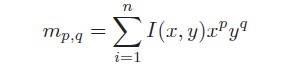
\includegraphics[scale=0.5]{images/moment.jpg}
  %\caption{sec }
%  \end{center}
%  \end{figure}
\end{itemize}
\vspace{0.5 cm}
\item From moment the centroid (CoG) is found.
\end{itemize}
\end{frame}

%\begin{frame}{Hand Tracking contd..}
%\begin{itemize}
%\item From moment The CoG (Center of gravity) is obtained, considering the 1st order moment of x and y %and the 0th order moment. 
%\linebreak
%\item The CoG (X, Y ) of the hand/palm region.
%\begin{figure}
%  \begin{center}
%  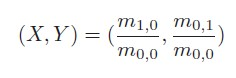
\includegraphics[scale=0.5]{images/Cog.jpg}
%  %\caption{sec }
%  \end{center}
%  \end{figure}
%\end{itemize}
%\end{frame}

\begin{frame}{PROPOSED SYSTEM}
\vspace{0.5cm}
 \begin{itemize}
\item Any hand gesture recognition system requires some basic
stages. These stages are
\vspace{.5 cm}
 \begin{itemize}
\item Gesture module and image acquisition
\item Hand segmentation
\item Tracking
\item \alert{Feature extraction}
\item Classification

\end{itemize}
\end{itemize}
\end{frame} 

\begin{frame}{Feature Extraction}

\begin{itemize}
\item Transforming the input data set into a set of
features is called feature extraction.
\linebreak
\item Considered data of 128 sample points as the feature set for each isolated gesture and data of 256 sample points as the
feature set for each continuous gesture.
\end{itemize}

\end{frame}

\begin{frame}{Feature Extraction}
\begin{itemize}
\item The extraction features are
\linebreak
\begin{itemize}
\item Orientation.
\linebreak
\item Gesture trajectory length,
\linebreak
\item Velocity and acceleration.
\end{itemize}
\end{itemize}
\end{frame}

\begin{frame}{Feature Extraction}
\begin{itemize}
\item Orientation 
\begin{itemize}
 \item Input is the sequence of centroids.
 \linebreak
 \item orientation feature can be calculated from a coordinate
geometrical formula.
\linebreak
\item Each angle is then converted into one of the eight directions
codes.
\begin{figure}
  \begin{center}
  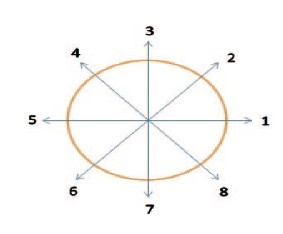
\includegraphics[scale=0.5]{images/ori1.jpg}
  %\caption{sec }
  \end{center}
  \end{figure}

%\item For every consecutive pair of points
%pi(xi, yi) and pi−1(xi−1, yi−1) (where i = 1,2,. . . ,N and
%N being the total number of points on the trajectory), the
%changing angle (θi) is given by
%\begin{figure}
%  \begin{center}
%  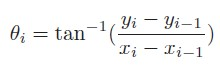
\includegraphics[scale=0.5]{images/orientation.jpg}
%  %\caption{sec }
%  \end{center}
%  \end{figure}
  

\end{itemize}
\end{itemize}
\end{frame}




\begin{frame}{Feature Extraction}
\begin{itemize}
\item Gesture trajectory length
\linebreak
\begin{itemize}
\item This feature is extracted by
considering the centre of gravity (CoG) of the trajectory to be
the point of reference from which the distance of other points
on the trajectory is found out.
\linebreak
%\item for every point
%(xi, yi) on the trajectory, the CoG (x', y') is calculated
%
%\begin{figure}
%  \begin{center}
%  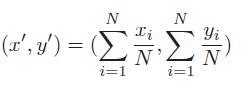
\includegraphics[scale=0.5]{images/trej1.jpg}
%  %\caption{sec }
%  \end{center}
%  \end{figure}
%  N is the total number of trajectory.
  
\end{itemize}
\end{itemize}
\end{frame}

%\begin{frame}{Feature Extraction contd..}
%\begin{itemize}
%\item The distance (Li) of every point (xi, yi) on the gesture
%trajectory from the CoG (x', y') is given by,
%\begin{figure}
%  \begin{center}
%  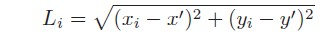
\includegraphics[scale=0.5]{images/trej2.jpg}
%  %\caption{sec }
%  \end{center}
%  \end{figure}
%  \item The normalized pattern size (Lavg) is given by,
%  \begin{figure}
%  \begin{center}
%  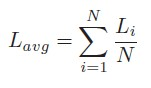
\includegraphics[scale=0.5]{images/trej3.jpg}
%  %\caption{sec }
%  \end{center}
%  \end{figure}
%  N is the total number of points on the gesture
%trajectory.
%  
%\end{itemize}
%\end{frame}
%
%\begin{frame}{Feature Extraction contd..}
%\begin{itemize}
%\item The total gesture trajectory length (L)
% \begin{figure}
%  \begin{center}
%  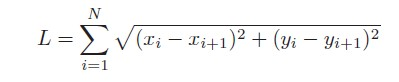
\includegraphics[scale=0.5]{images/trej4.jpg}
%  %\caption{sec }
%  \end{center}
%  \end{figure}
%  N is the total number of points on the gesture
%trajectory, (xi, yi) and (xi+1, yi+1) are the consecutive points
%on the gesture trajectory.
%\end{itemize}
%\end{frame}
%
%\begin{frame}{Feature Extraction contd..}
%\begin{itemize}
%\item trajectory length is size-normalized as pattern size for
%the same gesture alphabet may not be the same every time a
%gesture is performed, even by the same gesturer. This length
%(Lnormalized) is given by,
%\linebreak
% \begin{figure}
%  \begin{center}
%  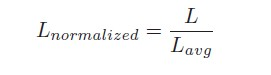
\includegraphics[scale=0.5]{images/trej5.jpg}
%  %\caption{sec }
%  \end{center}
%  \end{figure}
%\end{itemize}
%\end{frame}
%
%\begin{frame}{Feature Extraction contd..}
%\begin{itemize}
%\item Velocity and acceleration
%\begin{itemize}
%\item In coordinate geometry, velocity is
%nothing but the time rate of change of Euclidean distance.
%\begin{figure}
%  \begin{center}
%  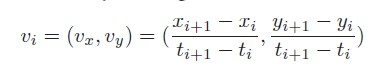
\includegraphics[scale=0.5]{images/vel1.jpg}
%  %\caption{sec }
%  \end{center}
%  \end{figure}
%  where vi is the velocity associated with neighbouring points
%(xi, yi) and (xi+1, yi+1) on the trajectory, ti and ti+1 denote
%the time instants and i= 1,2,. . . ,N.
%\end{itemize}
%\end{itemize}
%\end{frame}

\begin{frame}{Feature Extraction}
\begin{itemize}
\item Velocity and acceleration
\begin{itemize}
\item each alphabets the
velocity and the acceleration of change and transition is different.
\linebreak
\item Acceleration (a) is time derivative of velocity.
\linebreak
\item The acceleration and velocity are together considered. 
%\begin{figure}
%  \begin{center}
%  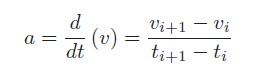
\includegraphics[scale=0.5]{images/vel2.jpg}
%  %\caption{sec }
%  \end{center}
%  \end{figure}
%  where vi+1 and vi are velocities at time instants ti+1 and
%ti, respectively.
\end{itemize}
\end{itemize}
\end{frame}

\begin{frame}{PROPOSED SYSTEM}
\vspace{0.5cm}
 \begin{itemize}
\item Any hand gesture recognition system requires some basic
stages. These stages are
\vspace{.5 cm}
 \begin{itemize}
\item Gesture module and image acquisition
\item Hand segmentation
\item Tracking
\item Feature extraction
\item \alert{Classification}

\end{itemize}
\end{itemize}
\end{frame} 

\begin{frame}{Classifier}
\begin{itemize}
\item Classifiers are those systems which accept feature set
as input and provide class-labeled output[1].
\linebreak
\item A
multilayer perceptron artificial neural network (MLP-ANN)
and focused time delay neural network (FTDNN)is considered.

\end{itemize}
\end{frame}

\begin{frame}{Classifier}
\begin{itemize}
\item MLP is a feed-forward ANN which is trained with back
propagation algorithm.
\linebreak
\item The MLP used in the work is a 3
layered network for both isolated and continuous gestures.
\linebreak
\begin{itemize}
\item Inputlayer
\item Hidden layer
\item Output layer
\end{itemize}
\end{itemize}
\end{frame}

%\begin{frame}{Classifier contd..}
%\begin{itemize}
%\item The perceptron control of wieghts, the summation processor and an activation fuction.
%\item Perceptron takes weighted sum of i/p s and o/p
%\begin{itemize}
%\item if(sum greater than threshold)   -- 1
%\item else --- 0
%\end{itemize}
%\item works, the inputs are presented to preceptron and if the output is same as desired output, satisfactory no change to the weights.
%\item else, weights need to be changed.
%\end{itemize}
%\end{frame}


\begin{frame}{Classifier}

\begin{figure}
  \begin{center}
  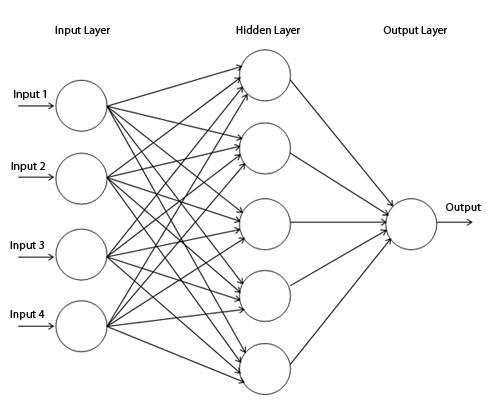
\includegraphics[scale=0.5]{images/MLP.jpg}
  %\caption{sec }
  \end{center}
  \end{figure}

\end{frame}

%\begin{frame}{Classifier contd..}
%\begin{itemize}
%\item Back propagation is used output to adjust the weights of inputs and output layer.
%\linebreak
%\item Also calculate the error at the previous layer and use to adjust the weights.
%\end{itemize}
%\end{frame}

%\begin{frame}{Classifier contd..}
%\begin{itemize}
%\item MLP is a feed-forward ANN which is trained with back
%propagation algorithm.
%\linebreak
%\item The MLP used in the work is a 3
%layered network for both isolated and continuous gestures.
%\linebreak
%\begin{itemize}
%\item Inputlayer
%\item Hidden layer
%\item Output layer
%\end{itemize}
%\end{itemize}
%\end{frame}

\begin{frame}{Classifier}
\begin{itemize}
\item The input layer contains 128 nodes for isolated gestures.
\linebreak
\item 256 nodes for continuous gestures
\linebreak
\item one input node per sample
point per gesture.



\end{itemize}
\end{frame}


%\begin{frame}{Classifier}
%\begin{itemize}
%\item The MLP is a feed forward ANN which trained by back propagation algorithm.
%\linebreak
%\item Has 3 layers 
%\linebreak
%\begin{itemize}
%\item Input layer (128 nodes for isolated gestures and
%256 nodes for continuous gestures)
%\item hidden layer (16 nodes)
%\item output layer (for each class of characters here 7)
%\end{itemize}
%


%\end{itemize}
%\end{frame}

\begin{frame}{Classifier}
\begin{itemize}

\item output layer contains as many
nodes as the number of classes of alphabets.
\linebreak
\item The maximum number of epochs chosen is 200
and minimum square error (mse) goal is 0.0001.
\linebreak



\end{itemize}
\end{frame}

\begin{frame}{Classifier}
\begin{itemize}
\item TDNN
\begin{itemize}
\item Multilayer feed forward neural network whose hidden and output layers are replicated across time.
\linebreak
\item The FTDNN, focus in the sense that the entirely network structure is located at the input end of the unit[3].
\linebreak
\item Use tapped-delay line with delays from
1 to 8 with 10 neurons in the hidden layer. The maximum
number of epochs chosen is 500 and mse goal is 0.0001.
\end{itemize}


\end{itemize}
\end{frame}

\begin{frame}{Classifier}
\begin{figure}
\begin{center}
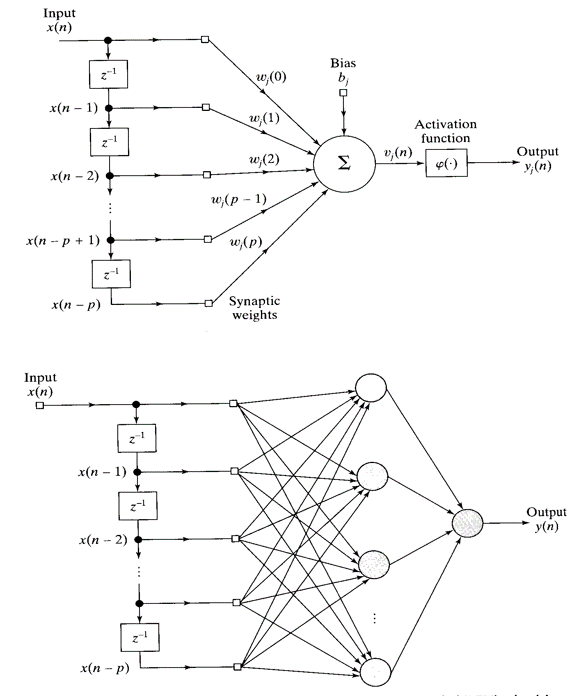
\includegraphics[scale=0.3]{Picture1.png}
\end{center}
\end{figure}
\end{frame}

\section{PROPOSED GESTURE RECOGNITION
METHODOLOGY}
\begin{frame}{PROPOSED GESTURE RECOGNITION
METHODOLOGY}

\begin{figure}
  \begin{center}
  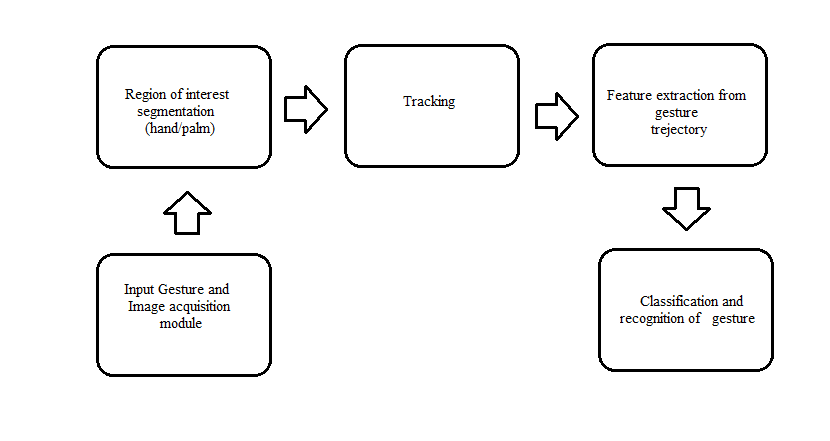
\includegraphics[scale=0.55]{images/modues.png}
  \caption{Block diagram for hand gesture recognition system }
  \end{center}
  \end{figure}

\end{frame}



\begin{frame}{PROPOSED GESTURE RECOGNITION
METHODOLOGY}
\begin{itemize}
\item The steps in SLR system are,

\begin{enumerate}


\item The captured RGB frame which is the input frame
here is first converted into the corresponding HSV and YCbCr
frame which are the outputs in this step[4].
\item Skin pixels are extracted by skin thresholding
applied on both the frames obtained from Step 1 to result in
skin-colour thresholded frames.
\item Both the frames obtained from Step 2 are then
converted into binary frames which contain pixel value either
0 or 1 and these binary frames are the outputs of this step
which contain only the contour of the segmented hand.
\item Morphological operations (e.g erosion, dilation etc)
are performed on the frames obtained in Step 3 to remove
unwanted noisy pixels.
\end{enumerate}
\end{itemize}
\end{frame}


\begin{frame}{PROPOSED GESTURE RECOGNITION
METHODOLOGY}
\begin{itemize}
\item The steps in SLR system are,
\begin{enumerate}
\setcounter{enumi}{4}
\item Logical AND operation is performed between the
planes obtained from Step 4 to remove the background noise
and to get the most-connected regions in the planes.
\item Centroid of segmented hand portion is calculated
and found from the frames obtained in Step 5 using moment
calculation[4].
\item Gesture trajectories are found by connecting the
centroids of the segmented hand during the gesticulation at
different time instants which results in the gesture alphabets
we intend to draw.
\item The features already mentioned are found out for
each gesture alphabet.
\item The feature vectors are then used as input to MLP
and FTDNN classifiers for recognition of the gesture alphabets.
\end{enumerate}
\end{itemize}


\end{frame}

%\begin{frame}{PROPOSED GESTURE RECOGNITION
%METHODOLOGY}
%\begin{itemize}
%\item the
%Gesture trajectories may be noisy due to the following reasons:
%\linebreak
%\begin{itemize}
%\item Hand trembling or undesired yet unavoidable hand
%movement causes the deviation of actual centroids.
%\linebreak
%\item  Due to change in hand shape, the actual centroids may
%be a little bit or significantly far away from the actual
%trajectories.
%\end{itemize}
%
%\end{itemize}
%\end{frame}
%
%
%\begin{frame}{PROPOSED GESTURE RECOGNITION
%METHODOLOGY}
%\begin{itemize}
%\item Solved by removing the
%isolated noisy points in the gesture path with a threshold value.
%\item a noisy point (xt, yt) is replaced
%by (x't, y't)
%\begin{figure}
%  \begin{center}
%  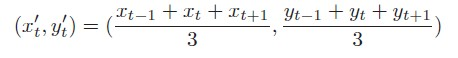
\includegraphics[scale=0.5]{images/noice.jpg}
%  %\caption{sec }
%  \end{center}
%  \end{figure}
%
%
%
%\end{itemize}
%\end{frame}


\begin{frame}{PROPOSED GESTURE RECOGNITION
METHODOLOGY}
\begin{itemize}
\item Recognition of Continuous Gestures
\linebreak
\begin{itemize}
\item The detection and recognition techniques involved with
continuous gestures are different from that of isolated gestures. 
\linebreak
\item In case of continuous recognition the time interval between 2 gestures must be know.
\linebreak
\item Here is take velocity of the actions is constant ie, acceleration is 0.

%%\item selected a suitable threshold value(aT) for acceleration , ie + ve for acceleration and -ve for de-acceleration.  
\end{itemize}
\end{itemize}
\end{frame}

\begin{frame}{PROPOSED GESTURE RECOGNITION
METHODOLOGY}
\begin{itemize}

\item After extracting the boundary information in the continuous
gestures with the help of acceleration feature, the neural
network have been
trained with these information to recognize these gestures.
\linebreak 
\item Here 30 samples video for training.  

\end{itemize}
\end{frame}

%\section{Experimental Results}
%
%\begin{frame}{Experimental Results}
%\begin{itemize}
%
%\item Hand segmentation
%\begin{figure}
%  \begin{center}
%  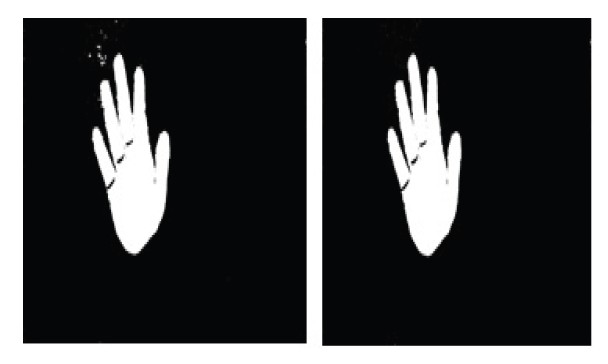
\includegraphics[scale=0.5]{images/segment.jpg}
%  %\caption{sec }
%  \end{center}
%  \end{figure}
%
%\end{itemize}
%\end{frame}
%
%\begin{frame}{Experimental Results}
%\begin{itemize}
%
%\item Tracking Results of Gestures
%\begin{figure}
%  \begin{center}
%  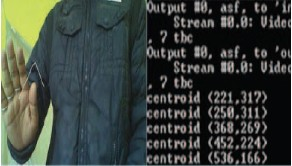
\includegraphics[scale=0.5]{images/centroid.jpg}
%  \caption{Gesture alphabet ‘A’ (left) and its tracking result (right)}
%  \end{center}
%  \end{figure}
%
%\end{itemize}
%\end{frame}
%
%
%\begin{frame}{Experimental Results}
%\begin{itemize}
%
%\item Isolated and Continuous Gestures
%\linebreak
%\item Isolated gestures ‘A’, ‘B’,
%‘C’, ‘D’, ‘E’, ‘F’, ‘O’ and ‘Q’ and six continuous gestures
%‘BA’, ‘AD’, ‘CA’, ‘CB’, ‘CF’ and ‘DB’ are considered.
%\begin{figure}
%  \begin{center}
%  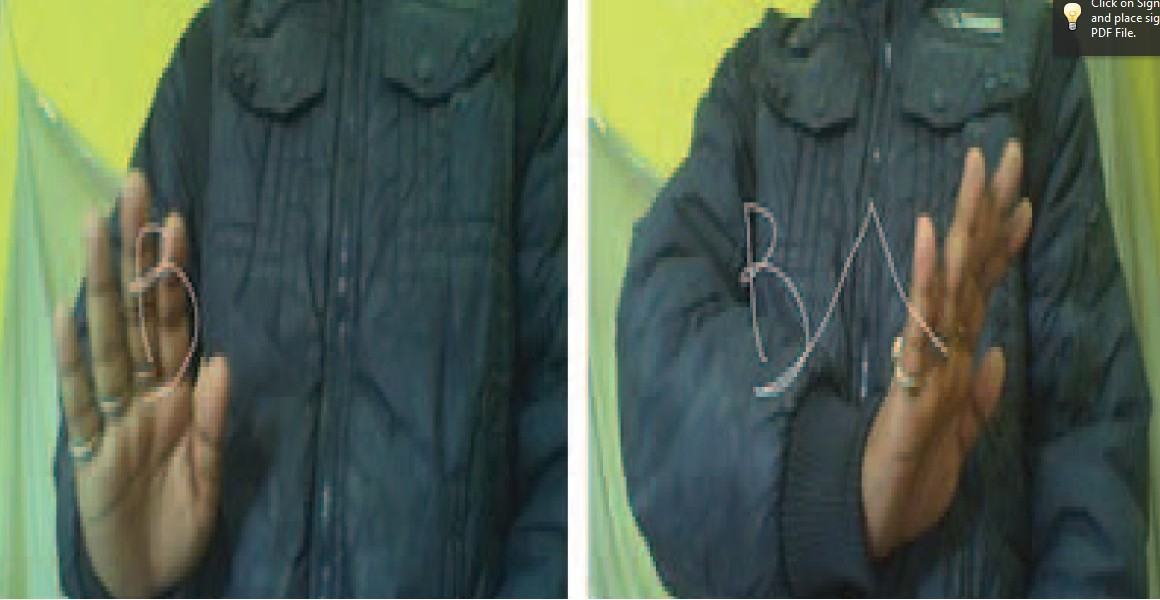
\includegraphics[scale=0.2]{images/user.jpg}
%  \caption{Isolated gesture ‘B’ (left) and continuous gesture ‘BA’
%(right)}
%  \end{center}
%  \end{figure}
%
%\end{itemize}
%\end{frame}
\section{CONCLUSION}
\begin{frame}{CONCLUSION}
\begin{itemize}
\item Provide
some insights into certain methods to recognize isolated and continuous English alphabets
hand gestures.
\linebreak
\item Here the system uses both MLP and FTDNN
\linebreak
\item The recognition
rate achieved with MLP in this case is 89.05 while that achieved with FTDNN is 87.14 
%\cite{hmm} \cite{ANN} \cite{site} \cite{book} \cite{site}
\end{itemize}
\end{frame}
\section{REFERENCES}
\begin{frame}[allowframebreaks]
\frametitle{REFERENCES}
    {\bibliographystyle{IEEEtran} }
    \bibliography{sample}
\end{frame}
\section{}
\begin{frame}
\begin{figure}
\begin{center}

\includegraphics[scale=0.7]{thankyou.png}
\end{center}
\end{figure}
\end{frame}



%------------------------------------------------



%----------------------------------------------------------------------------------------

\end{document} 